\documentclass[11pt, a4paper]{book}
\usepackage[french]{babel}
\usepackage[utf8]{inputenc}
\usepackage{answers}

\usepackage{hyperref}
\usepackage{multicol}

\usepackage[table,xcdraw]{xcolor}
\usepackage{listings}
\definecolor{ForestGreen}{RGB}{34,139,34}


\usepackage{enumitem}

\AtBeginDocument{\def\labelitemi{$\bullet$}}


\newcommand{\py}{\lstinline{Python} }


\definecolor{backcolour}{rgb}{0.95,0.95,0.92}

\lstset{%
	language         = Python,
	backgroundcolor  = \color{backcolour},
	basicstyle       = \ttfamily, % \upshape\ttfamily,
	keywordstyle     = \bfseries\color{blue}, %\bfseries,
	stringstyle      = \color{magenta},
	commentstyle     = \color{ForestGreen},
	alsoletter = > ,
	morekeywords = {>>>,as,assert,False,None, nonlocal,True, with,yield , <<, >>, :},
	showstringspaces = false,
	numbers=left,
	stepnumber=1,
	literate={à}{{\`{a}}}1 {é}{{\'e}}1 {è}{{\`{e}}}1 {ê}{{\^{e}}}1 {Ê}{{\^{E}}}1 {î}{{\^i}}1 {ô}{{\^{o}}}1 {ç}{{\c{c}}}1 {Ç}{{\c{C}}}1
}

\newcommand{\itemb}[1]{\item \textbf{#1}}

\usepackage{fancyhdr}  %package pour en-tetes et pied de pages
\usepackage{sectsty} % Permet de faire des modifications de police dans diverses sections des "headings" (cf. modif presentation de la page)
\pagestyle{fancy}       %Style pour en-tetes et pieds de pages
\fancyhead[CO,CE]{\sc Série 1\hspace{0.5mm}}
\fancyhead[RO,LE]{Collège Sismondi}  % LaTeX/TEX define \strut to be an invisible box of width zero that extends just enough above and below the baseline. Cela permet d'augementer légèrement la taille en bas de la box de manière à ce qu'elle soit collée à la ligne.
\fancyhead[LO,RE]{\small\ \textsl{1\textsuperscript{ère} année - DO Informatique}}
\fancyfoot[RO,LE]{2021 - 2022}
\fancyfoot[LO,RE]{\small }
\fancyfoot[CO,CE]{\thepage}

\fancyhfoffset[l]{1.2cm} % le "l" en paramètre permet d'indiquer qu'on ne veut modifier que la marge à gauche.
\renewcommand{\headrule}{{%
		\hrule \headwidth \headrulewidth \vskip-\headrulewidth}}
\renewcommand\footrulewidth{\headrulewidth}
\renewcommand{\footrule}{{%
		\vskip-\footruleskip\vskip-\footrulewidth
		\hrule \headwidth \footrulewidth\vskip\footruleskip}}

\usepackage{tikz}
%-------------------------------------------------------------------------------
%---- Eclairage : en encadré sur fond jaune avec symbôle "ampoule" à gauche ----
%-------------------------------------------------------------------------------
\definecolor{coleclairage}{RGB}{255 , 221 , 156}
\definecolor{contoureclairage}{RGB}{255 , 192 , 0}
\newenvironment{eclairage}
{
	\begin{center}%
		\begin{tikzpicture}%
			\node[rectangle, draw=contoureclairage, top color=coleclairage!50, bottom color=coleclairage!140, rounded corners=5pt, inner xsep=5pt, inner ysep=6pt, outer ysep=10pt]\bgroup                     
			\begin{minipage}{0.98\linewidth}
				\begin{minipage}{0.08\linewidth}\centerline{
\includegraphics[scale=1]{Symbole_eclairage.png}}\end{minipage}
				\begin{minipage}{0.89\linewidth}\itshape\footnotesize
				}
				{                		
				\end{minipage}
			\end{minipage}\egroup;%
		\end{tikzpicture}%
	\end{center}%
}

%-------------------------------------------------------------------------------
%---- apprendre : en encadré sur fond jaune avec symbôle "ampoule" à gauche ----
%-------------------------------------------------------------------------------
\definecolor{colapprendre}{RGB}{50,205,50}
\definecolor{contourapprendre}{RGB}{34,139,34}
\newenvironment{apprendre}
{
	\begin{center}%
		\begin{tikzpicture}%
			\node[rectangle, draw=contourapprendre, top color=colapprendre!10, bottom color=colapprendre!50, rounded corners=5pt, inner xsep=5pt, inner ysep=6pt, outer ysep=10pt]\bgroup                     
			\begin{minipage}{0.98\linewidth}
				\begin{minipage}{0.08\linewidth}\centerline{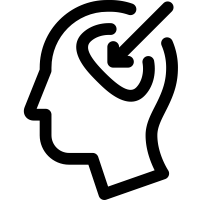
\includegraphics[width=30px]{Symbole_learn.png}}\end{minipage}
				\begin{minipage}{0.89\linewidth}\itshape\footnotesize
				}
				{                		
				\end{minipage}
			\end{minipage}\egroup;%
		\end{tikzpicture}%
	\end{center}%
}

\definecolor{colimportant}{RGB}{247 , 189 , 164}
\definecolor{contourimportant}{RGB}{237 , 125 , 49}
\newenvironment{important}
{
	\begin{center}%
		\begin{tikzpicture}%
			\node[rectangle, draw=contourimportant, top color=colimportant!50, bottom color=colimportant!140, rounded corners=5pt, inner xsep=5pt, inner ysep=6pt, outer ysep=10pt]\bgroup                     
			\begin{minipage}{0.08\linewidth}\centerline{
\includegraphics[scale=0.8]{Symbole_attention.png}}\end{minipage}
			\begin{minipage}{0.89\linewidth}
			}
			{                		
			\end{minipage}\egroup;
		\end{tikzpicture}%
	\end{center}%
}

%-----------------------------------------------------------------
%---- Modification présentation de la page: marges de la page ----
%-----------------------------------------------------------------
%\addtolength{\hoffset}{-1in}              % 1
%\addtolength{\voffset}{-1in}              % 2
\addtolength{\oddsidemargin}{-0.1 in} % 3
\addtolength{\evensidemargin}{-1in} % 3
\addtolength{\topmargin}{-1in}       % 4
\addtolength{\headheight}{6pt}       % 5
%\addtolength{\headsep}{-0.2cm}           % 6
\setlength{\textheight}{26cm}    % 7
\setlength{\textwidth}{16.5cm}      % 8
\addtolength{\marginparsep}{0pt}      % 9
\setlength{\marginparwidth}{0pt}   % 10
\addtolength{\footskip}{-1mm}           %11

\setlength{\parindent}{0em}% pas d'indentation


% Customiser le nom des sections
\usepackage{titlesec}
\titleformat{\section}[hang]{\Large \bfseries}{Série \thesection:\ }{0pt}{}

\renewcommand{\familydefault}{\sfdefault} % pour avoir des polices san serif

\newtheorem{Exc}{Exercice}
\Newassociation{correction}{Soln}{mycor}
\renewcommand{\Solnlabel}[1]{\bfseries Ex #1 }
\def\exo#1{%
	\futurelet\testchar\MaybeOptArgmyexoo}
\def\MaybeOptArgmyexoo{
	\ifx[\testchar \let\next\OptArgmyexoo
	\else \let\next\NoOptArgmyexoo \fi \next}
\def\OptArgmyexoo[#1]{%
	\begin{Exc}[#1]\normalfont}
	\def\NoOptArgmyexoo{%
		\begin{Exc}\normalfont}
		\newcommand{\finexo}{\end{Exc} \vspace{3mm}}
	\newcommand{\flag}[1]{}
	\newcommand{\entete}[1]

\newcommand{\getexocompteur}{{\the\numexpr \arabic{Exc}  \relax}}	
	
\newcommand{\eexo}{\vspace{5mm}} % espace pour séparer les exercices
\pgfplotsset{compat=1.17}

\begin{document}

\setcounter{chapter}{5}
\chapter{Structure de données finie et base de l'algorithmique}



\section{La variable}
\subsection{Définition}

\begin{defi}
Une {\it structure de données} est une structure logique destinée à stocker et organiser des données de façon à faciliter leur utilisation. Parmi ces structures, on retrouve la {\it variable}, le {\it tableau}, le {\it graphe}, l'{\it arbre}.... 
\end{defi}

En programmant en Makecode Microbit nous avons souvent fait appel à des variables. Nous allons maintenant les définir:

\begin{defi}
La {\it variable} est une structure de données finie. C'est un élément qui associe un nom (l'identifiant de la variable) à une valeur. Nous pouvons différencier la {\it constante} qui, une fois qu'une valeur lui a été attribuée, ne change plus, et la {\it variable mutable} qui elle peut changer de valeur tout au long du programme.

\end{defi}

\begin{remarque}
En Microbit, la variable est créée avant qu'une valeur ne lui soit attribuée. Pour régler ce problème, dès qu'une variable est créée, Microbit lui associe la valeur 0 par défaut.  La valeur peut être ensuite modifiée en utilisant le bloc:
\begin{center}
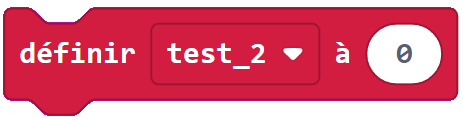
\includegraphics[scale=.5]{ch6_images/var_1}
\end{center}
\end{remarque}
	
	
	
\newpage
	
	
	
\begin{exercice}
 Regarder le programme suivant, et deviner ce qu'il va se passer quand on va activer le Microbit:

\begin{center}
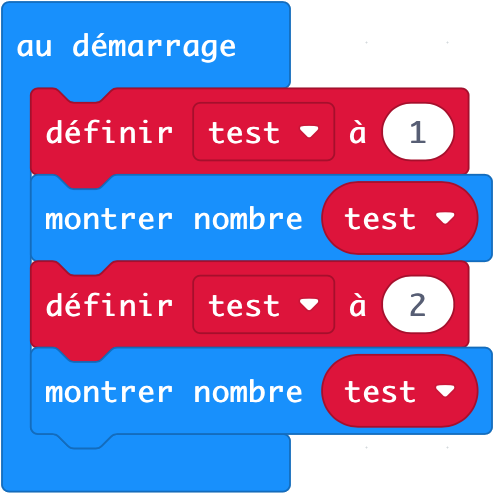
\includegraphics[scale=.6]{ch6_images/var_2}
\end{center}
\end{exercice}

\subsection{Nom d'une variable}
% Edoardo (14.11.2021)
Le nom choisi pour chaque variable est important pour facilité la lisibilité de votre programme. Il vous permet de vous souvenir du rôle de chaque variable. Imaginez des milliers de blocs d'instruction Microbit dans votre programme avec des centaines de variables. Si vous nommez vos variables avec des noms peu explicites comme v1, v2, v3, v4 ... v100 seriez-vous capable de retrouver à quoi sert chaque variable ?

Bien que nous soyons toujours libre d'écrire le nom d'une variable comme bon nous semble, un certain nombre de convention sont utilisées:
\begin{enumerate}[1)]
\item Un nom pertinent : essayez d'être le plus précis et concis possible, mais préférez la compréhension à la longueur du nom de la variable. 
\item Toujours commencer par une minuscule
\item Pas de caractères spéciaux ou d'accents
\item Si une variable est un mot composé, deux solutions s'offrent à vous :
\begin{enumerate}[a)] 
\item Notation {\it camel case} : voiciUnExemple. Chaque nouveau mot commence par une majuscule.
\item  Notation {\it snake case} : voici\_ un\_ exemple. Chaque nouveau mot est séparé par un {\it underscore}:\_.

\end{enumerate}
\end{enumerate}

\begin{exercice}
Parmi les noms de variables suivants, lesquels respectent les conventions d'écritures des variables?
\begin{enumerate}
\item laVariable
\item la variable
\item nom\_de\_famille
\item la\_quantité
\item nombreDeVoitures
\item prenom
\item leNumeroDeTelephone
\item le\_ Nom
\item iztrdr3fsfs

\end{enumerate}
\end{exercice}


\subsection{\'Evolution d'une variable}

En Microbit il existe deux façon de modifier une variable. La première consiste à lui attribuer une valeur, comme on l'a vu précédemment, avec le bloc {\it Définir variable à ...}:

\begin{center}
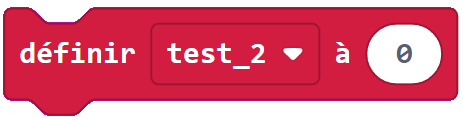
\includegraphics[scale=.4]{ch6_images/var_1}
\end{center}

L'autre façon de modifier une variable consiste à lui ajouter ou soustraire un certain nombre avec le bloc:

\begin{center}
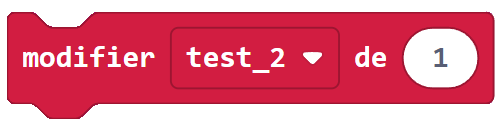
\includegraphics[scale=.4]{ch6_images/var_3}
\end{center}

On peut dire qu'on {\bf incrémente} la variable {\it test\_2}. {\bf Incrémenter} signifie ajouter une certaine valeur, souvent 1, à un nombre ou une variable. Dans le bloc précédent, la valeur de {\it test\_2} va changer et son contenu passera de 0 à 1. 

On parler de {\bf décrémenter} quand on soustrait une certaine valeur. Par exemple, dans le bloc suivant la variable {\it test\_2} qui valait 1, voit son contenu passer de 1 à 0.

\begin{center}

\includegraphics[scale=.4]{ch6_images/var_3a}
\end{center}

Il est aussi possible de mettre un calcul dans l'attribution d'une valeur à la variable. Le prochain bloc d'instruction définit la valeur de la variable {\it var\_1} au résultat du calcul $2+4$.

\begin{center}
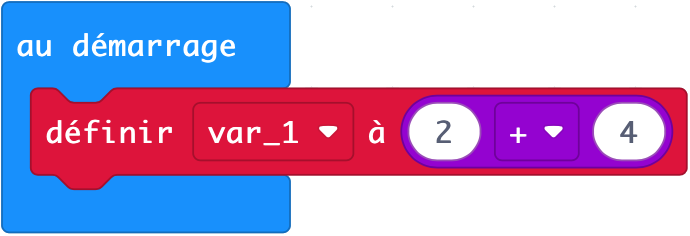
\includegraphics[scale=.5]{ch6_images/var_5}
\end{center}

Ou même d'utiliser la valeur de la variable elle-même:

\begin{center}
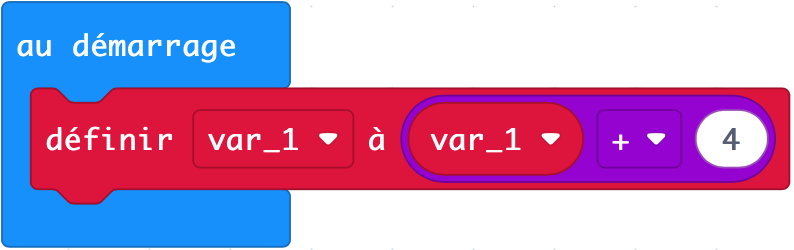
\includegraphics[scale=.5]{ch6_images/var_6}
\end{center}
Dans ce cas de figure, on additionne 4 au contenu de la {\it var\_1}. La variable {\it var\_1} verra ainsi sa valeur actuelle incrémentée de 4.

\begin{remarque}
Dans certains langages de programmation (comme par exemple Python), ce bloc s'écrirait:
$$var\_1=var\_1+4$$

\begin{enumerate}
\item Ce qui mathématiquement n'a pas de sens.
\item Le signe "=" n'a donc pas la même signification en informatique et en mathématique!
\item Il s’agit d’un symbole d’affectation (nous plaçons un certain contenu dans une variable) et non un symbole d’égalité.
\item Il faut le lire comme: {\it la variable var\_1 prend comme nouvelle valeur son ancienne valeur à laquelle on ajoute 4.} 
\end{enumerate}
\end{remarque}

Il est donc très important de comprendre cette finesse liée à la programmation !

\begin{exercice}
Quel nombre sera affiché par le programme?
\begin{center}
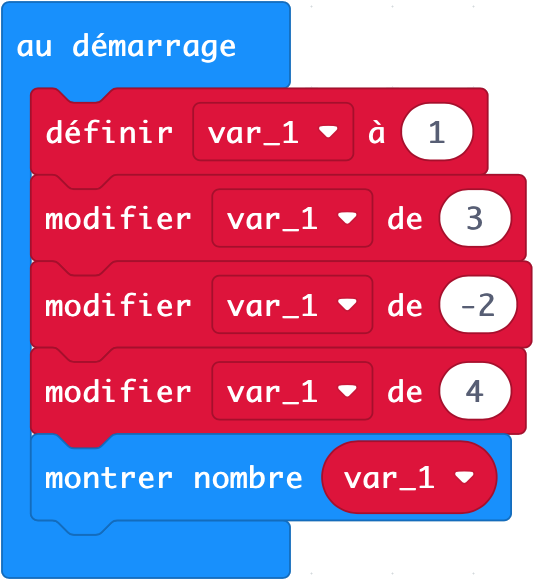
\includegraphics[scale=.5]{ch6_images/var_4}
\end{center}
\end{exercice}

\begin{exercice}
Quel nombre sera affiché par le programme?
\begin{center}
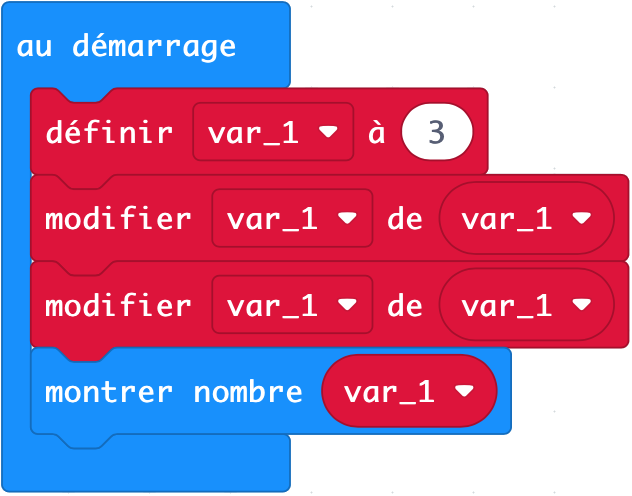
\includegraphics[scale=.5]{ch6_images/var_7}
\end{center}
\end{exercice}

\begin{exercice}
Quel nombre sera affiché par le programme?
\begin{center}
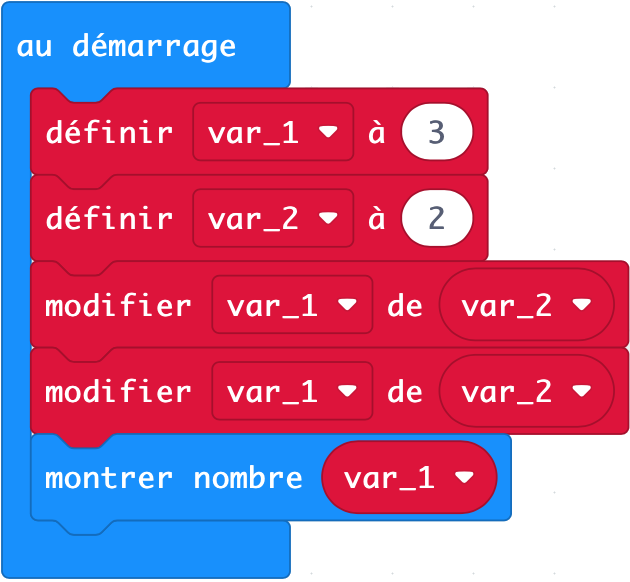
\includegraphics[scale=.5]{ch6_images/var_8}
\end{center}
\end{exercice}

\newpage

\begin{exercice}
Quels nombres seront affichés par le programme?
\begin{center}
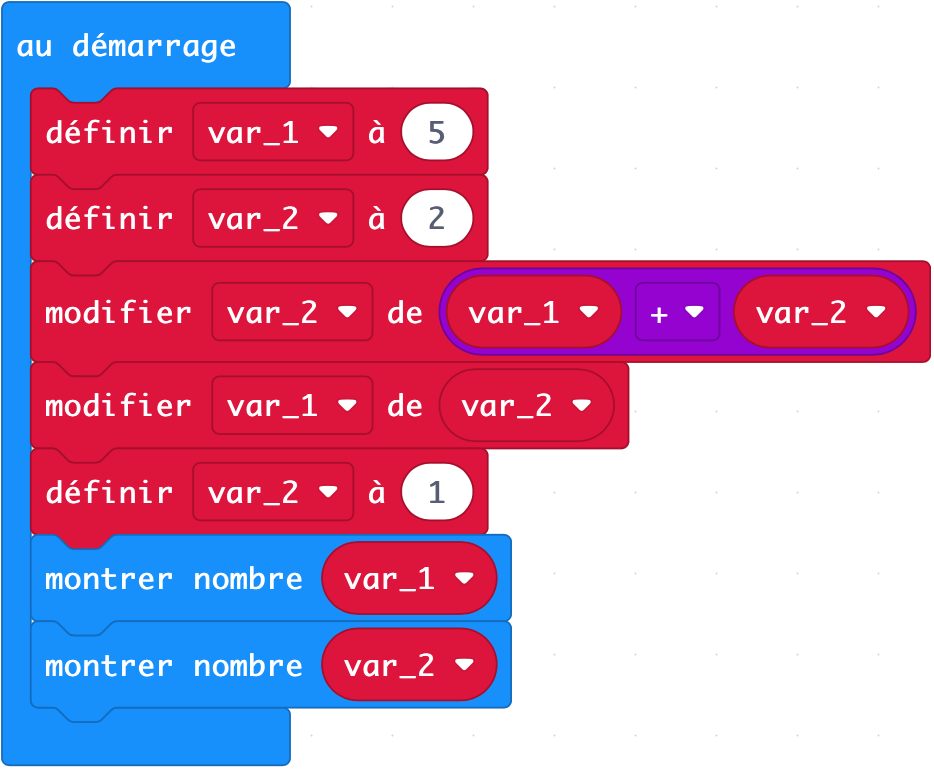
\includegraphics[scale=.5]{ch6_images/var_9}
\end{center}
\end{exercice}


\section{Les types}

\subsection{Motivation}

Une variable n'aura pas toujours comme valeur un nombre. Dans l'onglet {\it Texte} de Microbit, il est possible de choisir le symbole " " représentant une chaîne de caractères. Ainsi il est possible d'attribuer comme valeur une chaîne de caractère: 

\begin{center}
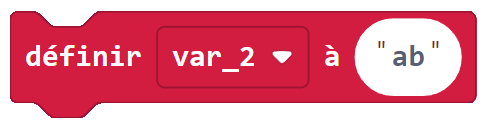
\includegraphics[scale=.4]{ch6_images/var_10}
\end{center}

Ainsi la variable {\it var\_2} est une chaîne de caractère. Essayons d'imaginer ce qu'il va se passer si nous faisons le programme suivant:

\begin{center}
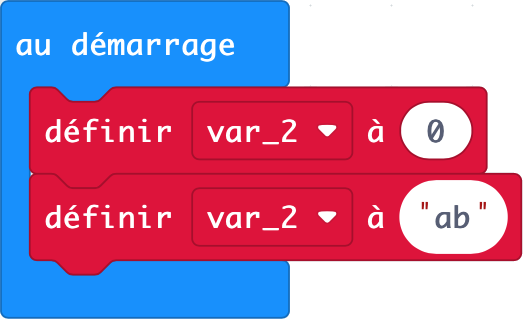
\includegraphics[scale=.5]{ch6_images/var_11}
\end{center}

Que se passe-t-il?

\vskip4cm

Lorsque Microbit repère un problème, il le signale. Dans l'exercice qui suit, essayer de comprendre le problème qui a été rencontré:

\begin{exercice}
Quel problème a été rencontré dans chacun de ces programmes?

\begin{center}
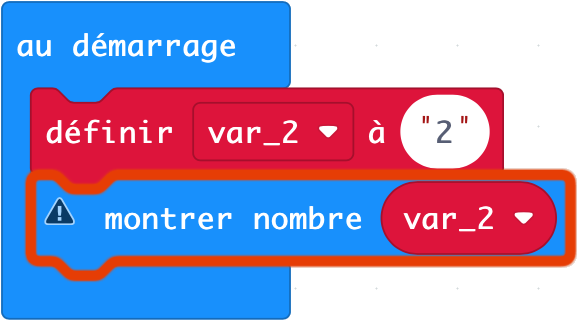
\includegraphics[scale=.5]{ch6_images/var_12}
\end{center}

\begin{center}
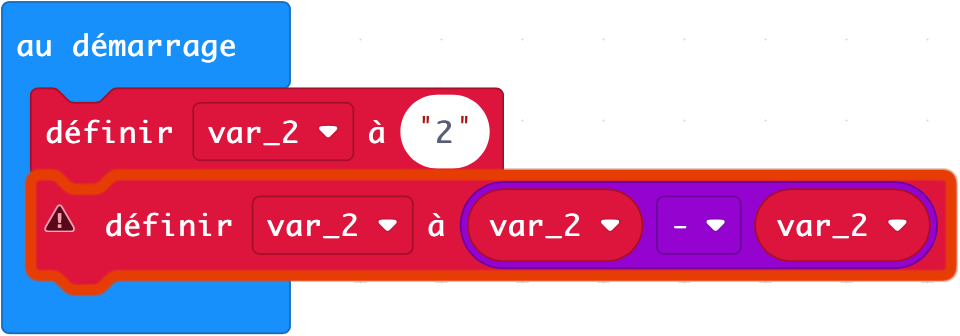
\includegraphics[scale=.5]{ch6_images/var_13}
\end{center}

\end{exercice}

\begin{remarque}
Chaque langage de programmation aura ses propres spécificités par rapport aux différents types d'erreurs qui peuvent apparaître. Par exemple, en Microbit, le programme ci-dessous fonctionne, et affiche 22!!

\begin{center}
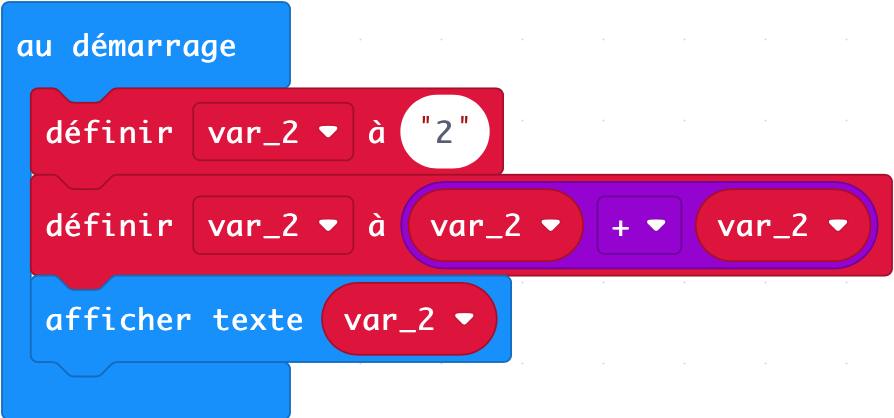
\includegraphics[scale=.5]{ch6_images/var_14}
\end{center}
\end{remarque}

\subsection{Définition}

On a vu que suivant la valeur attribuée à une variable, le programme va permettre de faire certaine action et en refuser d'autre. On définit cela formellement:

\begin{defi}
Le {\it type} d'une variable est l'interprétation que fera l'ordinateur de la valeur associée à cette variable. Ce type pourra être, entre autre, un nombre entier ({\it integer}), un nombre décimal ({\it float}), une chaîne de caractère ({\it string}), un booléen ({\it boolean})...
\end{defi}

Selon le langage de programmation que l'on utilise, le type d'une variable peut ou ne peut pas être changé. On parlera de {\bf typage statique} ou {\bf typage dynamique}. Par exemple, Microbit a un typage statique. Une variable définit comme un nombre ne peut plus être changé en une chaîne de caractères. 

On regarde maintenant chacun de ces types en détail. 



\subsection{Les types {\it entier} (integer) et {\it décimal} (float)}

La première catégorie de variables avec laquelle on aimerait travailler est le nombre. Cette catégorie se divise en 2 catégories principales. Comme nous l'avons vu, un nombre entier (positif ou négatif) n'utilise pas le même encodage qu'un nombre à virgule (qui utilise plutôt un encodage sous la forme d'une écriture scientifique). L'espace mémoire n'est donc pas le même. 

\begin{defi}
Le type {\it entier} (integer) caractérise une variable dont la valeur est un nombre entier. Le type {\it décimal} (float) caractérise une variable dont la valeur est un nombre décimal.
\end{defi}

Pour un programme, {\bf 1} sera un {\it entier} alors que {\bf 1.0} sera un {\it décimal}.

Pour Microbit, ainsi que pour de nombreux langages de programmation, il n'y a pas de problèmes à passer d'un nombre entier à un nombre décimal au cours du programme sans devoir changer de variable et de type.


\subsection{Le type {\it chaîne de caractères} (string)}

Une autre valeur que peut prendre une variable est la chaîne de caractères, ou le type {\it string}.

\begin{defi}
Le type {\it chaîne de caractères} (string) caractérise une variable dont la valeur est une suite de caractères. Cette suite peut aussi contenir des nombres qui sont alors interprétés comme des caractères.
\end{defi}

Le programme suivant n'a par exemple aucune signification pour Microbit:

\begin{center}
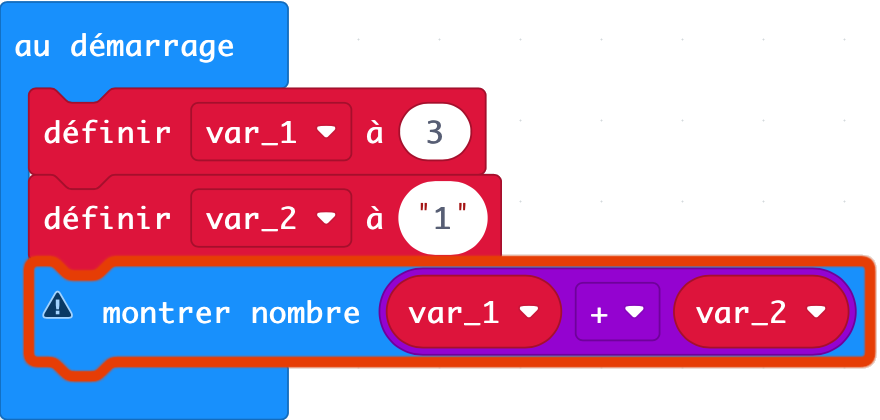
\includegraphics[scale=.5]{ch6_images/var_15}
\end{center}

Nous ne pouvons pas effectuer d'opération avec les chaînes des caractères (sauf le + que l'on verra par la suite). Il est par contre possible de comparer des chaînes de caractères:

\begin{center}
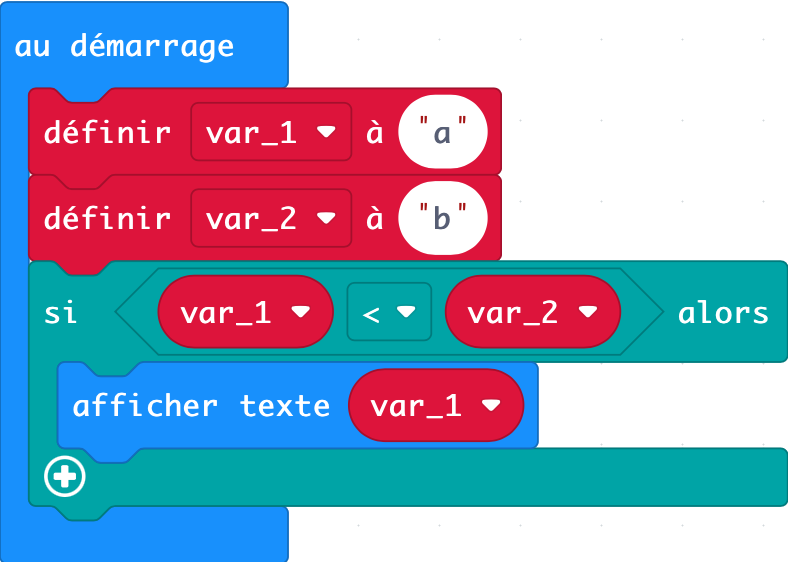
\includegraphics[scale=.5]{ch6_images/var_16}
\end{center}
Dans ce cas, comme la lettre a (contenu dans {\it var\_1}) se trouve avant b (contenu dans ({\it var\_2}) en prenant compte de l'ordre alphabétique, le texte contenu dans la {\it var\_1} s'affiche. Le Microbit affiche le texte a.

% Edoardo, 17.11.2021
Prenons un autre exemple:
\begin{center}
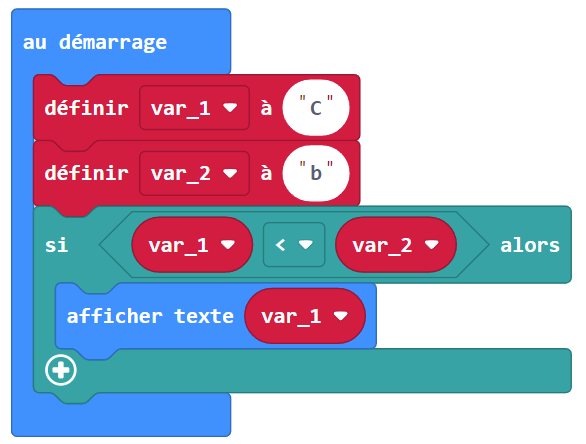
\includegraphics[scale=.5]{ch6_images/var_16a}
\end{center}
Dans ce cas, Microbit affiche C. Pourquoi le programme considère t'il que C est plus petit que b ? Tout simplement parce qu'il se base sur son code ASCII pour comparer ! Le code ASCII de C est 67 (base 10) alors que b est 98 (base 10).
% end Edoardo

\newline

L'opération principale sur les chaînes de caractères est la {\bf concaténation}:

\begin{defi}
La {\it concaténation} est une action qui prend en entrée plusieurs chaînes de caractères et renvoie une unique chaîne de caractères composée des différentes chaînes de caractères misent bout à bout.
\end{defi}

Par exemple, {\it concaténation("abc"; "d2")="abcd2"}.

\ 

Dans Microbit, l'opération + a le même effet que la concaténation si on lui donne deux chaînes de caractères. Ainsi, le programme suivant donnera "23":

\begin{center}
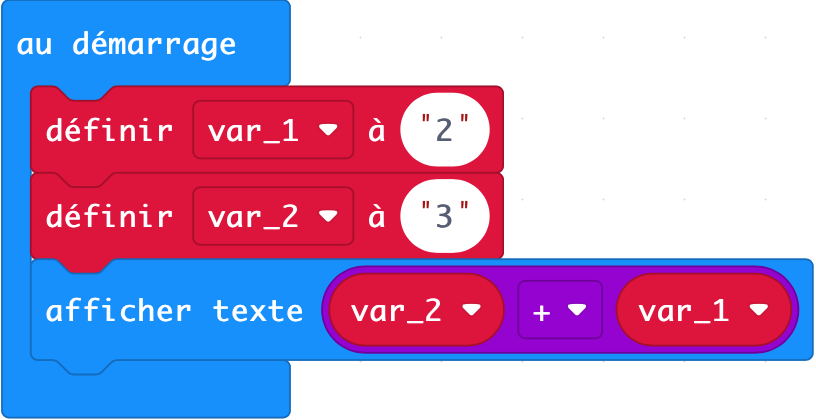
\includegraphics[scale=.5]{ch6_images/var_17}
\end{center}

Alors que le programme ci-dessous va afficher 5:

\begin{center}
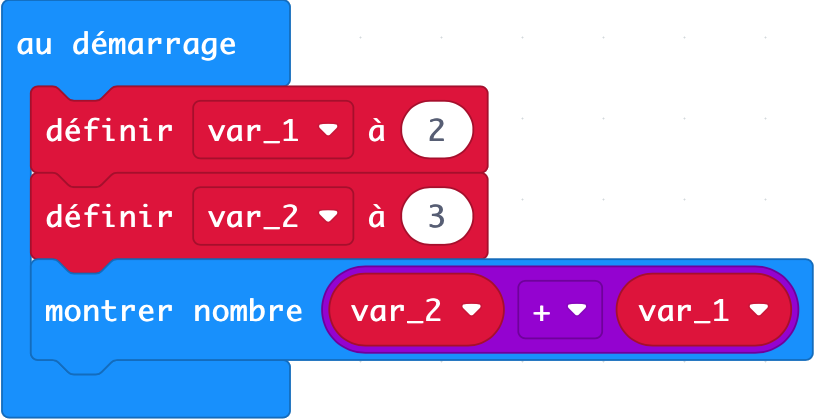
\includegraphics[scale=.5]{ch6_images/var_18}
\end{center}

\subsection{Le type {\it booléen}}

En informatique nous devons souvent tester une condition ("le nombre suivant est il pair?", "la variable vaut-elle 2?"...). Pour cela, nous avons besoin d'un type de variable qui ne correspondra ni à un nombre ni à une chaîne de caractères mais qui pourra nous permettre de résoudre un problème du type: si "il pleut", alors "il faut prendre un parapluie". Le test "il pleut" peut prendre deux valeurs: soit c'est vrai, soit c'est faux. C'est ce que nous appelons une {\bf variable booléenne}:

\begin{defi}
Le type {\it booléen} caractérise une variable qui peut avoir une des deux valeurs suivantes: "vrai" ou "faux".
\end{defi}

% Edoardo 27.11.2021
Dans Microbit, le type booléen est noté par un hexagone vert. Dans le cas suivant la variable {\it var\_1} est initialisée avec la valeur vrai ({\it true}).
\begin{center}
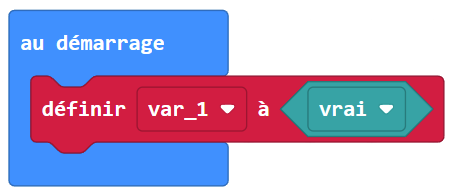
\includegraphics[scale=.5]{ch6_images/var_19a}
\end{center}
% End Edoardo

On remarque qu'une variable booléenne ne peut pas être affiché comme un nombre dans Microbit:

\begin{center}
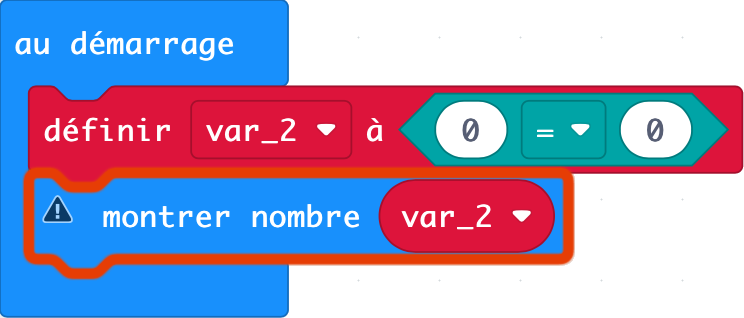
\includegraphics[scale=.5]{ch6_images/var_19}
\end{center}

Mais il peut être affiché comme un texte (le Microbit affiche {\it true} même si votre éditeur de code est configuré en français):

\begin{center}
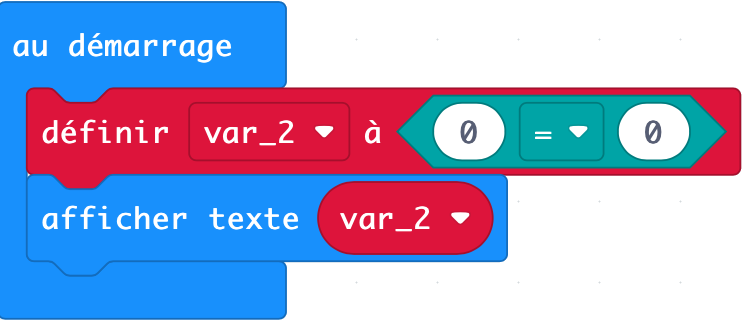
\includegraphics[scale=.5]{ch6_images/var_20}
\end{center}

\begin{exercice}
Définir quel type (entier, décimal, chaîne de caractères, booléen) devrait-on associer à une variable si cette variable représente:
\begin{enumerate}[a)]
\item l'âge d'une personne;
\item si il pleut;
\item un mois de l'année;
\item le prix d'un vêtement;
\item si une personne est majeure;
\item une année de naissance;
\item l'aire d'une forme géométrique;
\item le nom d'une personne;
\item si un végétal donné est un fruit;
\end{enumerate}
\end{exercice}



\begin{exercice}
Donner le type de chaque variable de ce programme puis dire si des erreurs vont être reconnues par Microbit (tester le programme si besoin):
\begin{center}
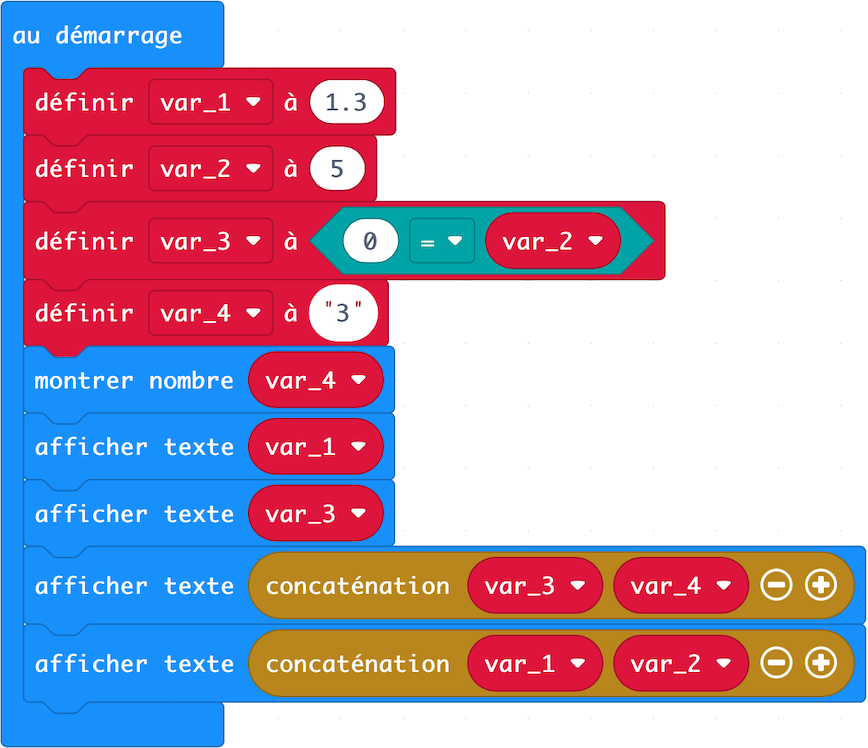
\includegraphics[scale=.7]{ch6_images/var_21}
\end{center}

\end{exercice}

\section{Bases de l'algorithmique}

Nous allons commencer à discuter ce que représente un algorithme et comment peut-on décomposer une tâche en tâches plus élémentaires dans le but de résoudre un problème ou d'accomplir un travail. La pensée algorithmique est un pan essentiel de l'informatique. Une fois correctement formulée ou précisée, elle permet, via un langage de programmation, d'implémenter différents traitements sur les machines (par exemple votre ordinateur).


\subsection{Définition}
\begin{defi}
Un algorithme est une suite finie et non-ambiguë d'opérations ou d'instructions permettant de résoudre un problème.

\end{defi}

On connaît depuis l'antiquité des algorithmes sur les nombres, comme par exemple l'algorithme d'Euclide qui permet de calculer le {\it pgdc}\footnote{pgdc: plus grand diviseur commun.} de deux nombres entiers.

Pour le traitement de l'information, on a développé des algorithmes opérant sur des données non numériques : les algorithmes de tri, qui permettent par exemple de ranger par ordre alphabétique une suite de noms, les algorithmes de recherche d'une chaîne de caractères dans un texte, ou les algorithmes d'ordonnancement, qui permettent de décrire la coordination entre différentes tâches, nécessaire pour mener à bien un projet.

Algorithme provient du nom du mathématicien perse {\it  Al-Khawarizmi} ($\sim$ 820), le père de l'algèbre.

\subsection{Les structures de contrôle}

Pour construire un algorithme, nous avons besoin d'une suite d'instructions. Ces instructions sont prises parmi un ensemble de {\it fonctions} (pour un langage de programmation) ou de {\it blocs} pour Microbit et sont exécutées les unes après les autres. Afin de {\it répéter} une même action un certain nombre de fois ou de faire une action {\it si} une condition est vraie, nous avons besoin de structure de contrôle:

\begin{defi}
Une {\it structure de contrôle } détermine dans quel ordre vont être exécutées les actions. Il en existe trois:
\begin{enumerate}
\item La {\it séquence}: les instructions sont effectuées les unes après les autres
\item La {\it séléction}: les instructions sont effectuées si une certaine
 condition est respectée (par exemple la structure {\it si})
\item La {\it répétition}: les instructions sont répétées en boucle {\it tant qu}'une certaine condition est respectée.
\end{enumerate}
\end{defi}

Ses structures sont récurrentes et apparaissent toujours sous une forme ou sous une autre dans presque tous les langages de programmation. Nous allons maintenant étudier les différentes structures qui sont à notre disposition.

\subsection{La condition {\it si} (if)}

Une des premières structures qui nous intéresse est la structure de sélection {\it si} ou {\it if} en anglais. Sa syntaxe en pseudo-code est de la forme:

\ 

\hskip5cm {\bf condition} 
	
\hskip+6cm alors {\bf action}

\ 

Le {\it si} vérifie si la {\bf condition} est {\it vraie} et si c'est le cas, la ligne avec l'{\bf action} est effectuée. La {\bf condition} est donc forcément un {\bf booléen} qui sera soit vrai soit faux.

Par exemple, on peut avoir le code suivant:

\ 

\hskip5cm {\it si} {\bf il pleut} 
	
\hskip+6cm alors {\bf je prends mon parapluie}

\ 

{\bf il pleut} est bien un booléen. Cela est soit vrai soit faux. Si cela est vrai, la ligne {\bf je prends mon parapluie} est exécutée. Si c'est faux, cette ligne ne sera pas évaluée. 

Pour un code Microbit, cela donnerait:

\begin{center}
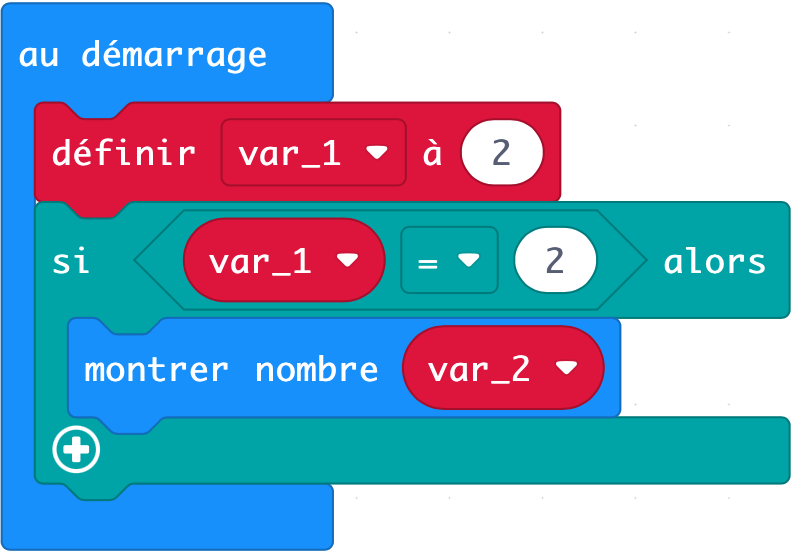
\includegraphics[scale=.45]{ch6_images/var_22}
\end{center}

Une condition {\it si} peut vérifier d'autres conditions, qui débutent par {\it sinon si} (else, if) et peut aussi finir par un {\it sinon} (else) qui ne sera exécuté que si toutes les autres conditions étaient fausses:

\ 

\hskip+5cm {\it Si} {\bf j'ai entre 500 et 1000 .-} 
	
\hskip+6cm alors {\bf je pars en Europe}

\hskip+5cm {\it sinon, si} {\bf j'ai entre 1000 et 2000 .-} 
	
\hskip+6cm alors {\bf je pars en Asie}

\hskip+5cm {\it sinon, si} {\bf j'ai plus que 2000.-} 
	
\hskip+6cm alors {\bf je pars en Amérique}

\hskip+5cm {\it sinon}  {\bf je reste chez moi}

\ 

Le programme équivalent en Microbit serait:

\begin{center}
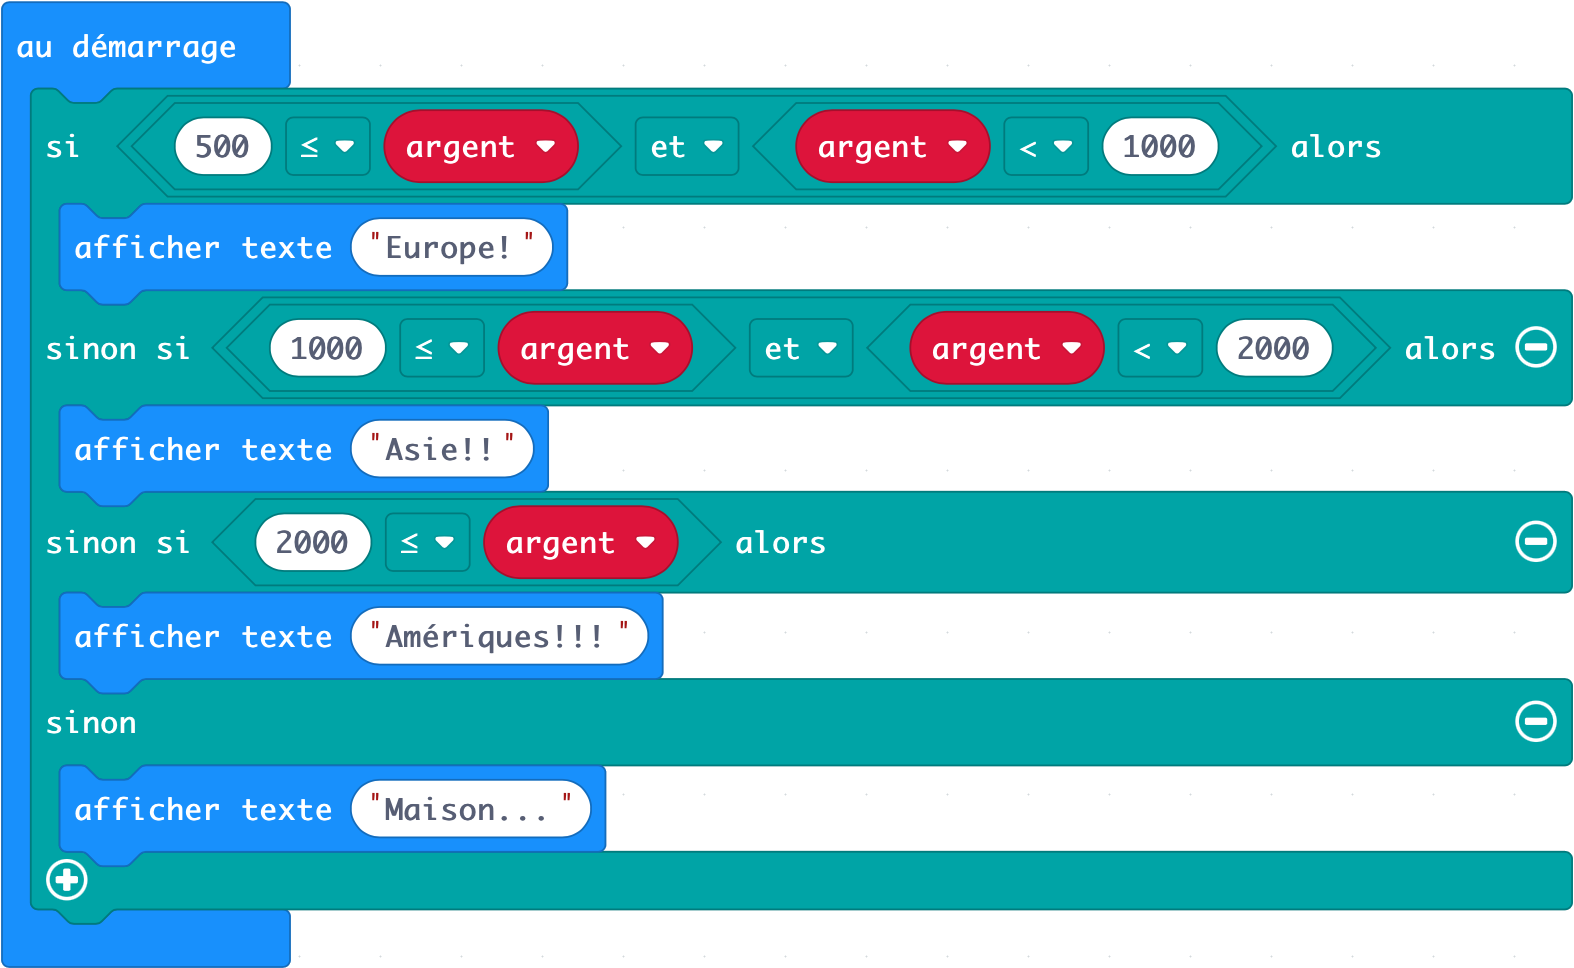
\includegraphics[scale=.5]{ch6_images/var_23}
\end{center}

\

\ 

\begin{exercice}
Que peut afficher ce programme?
\begin{center}
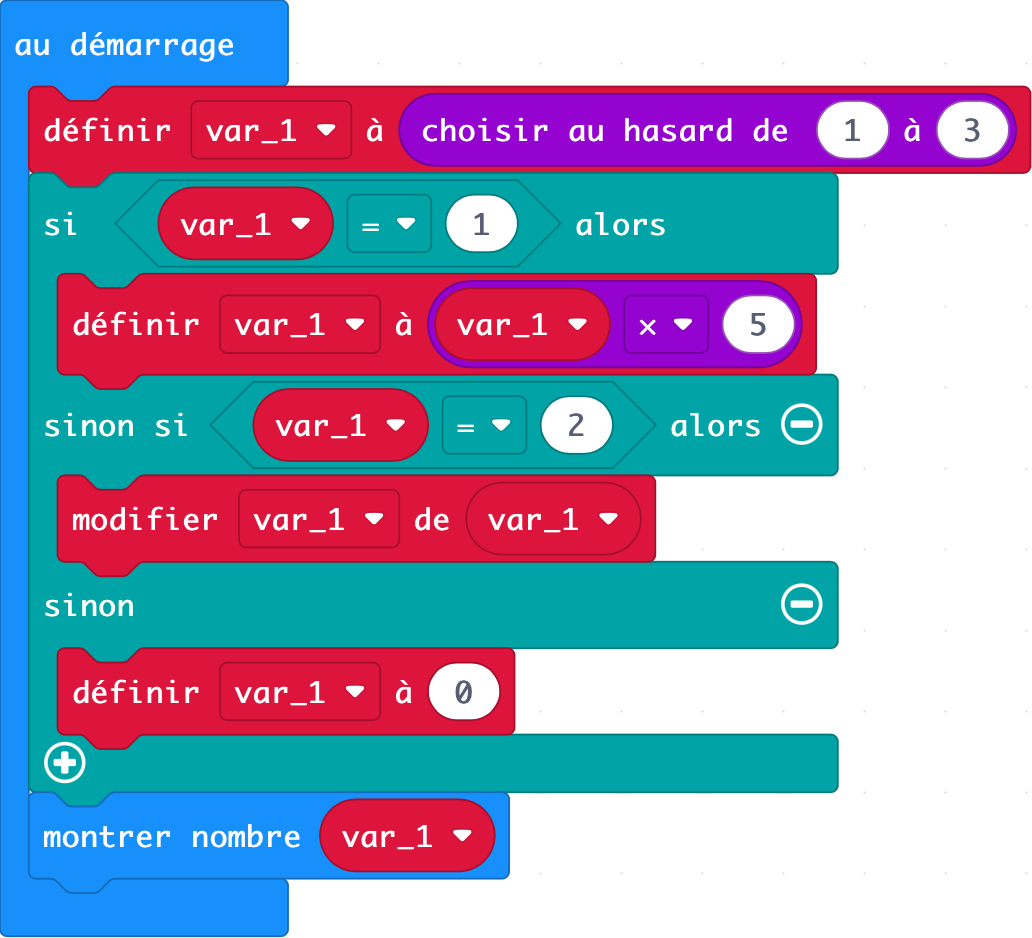
\includegraphics[scale=.5]{ch6_images/var_24}
\end{center}
\end{exercice}

\begin{exercice}
Qu'affiche ce programme?
\begin{center}
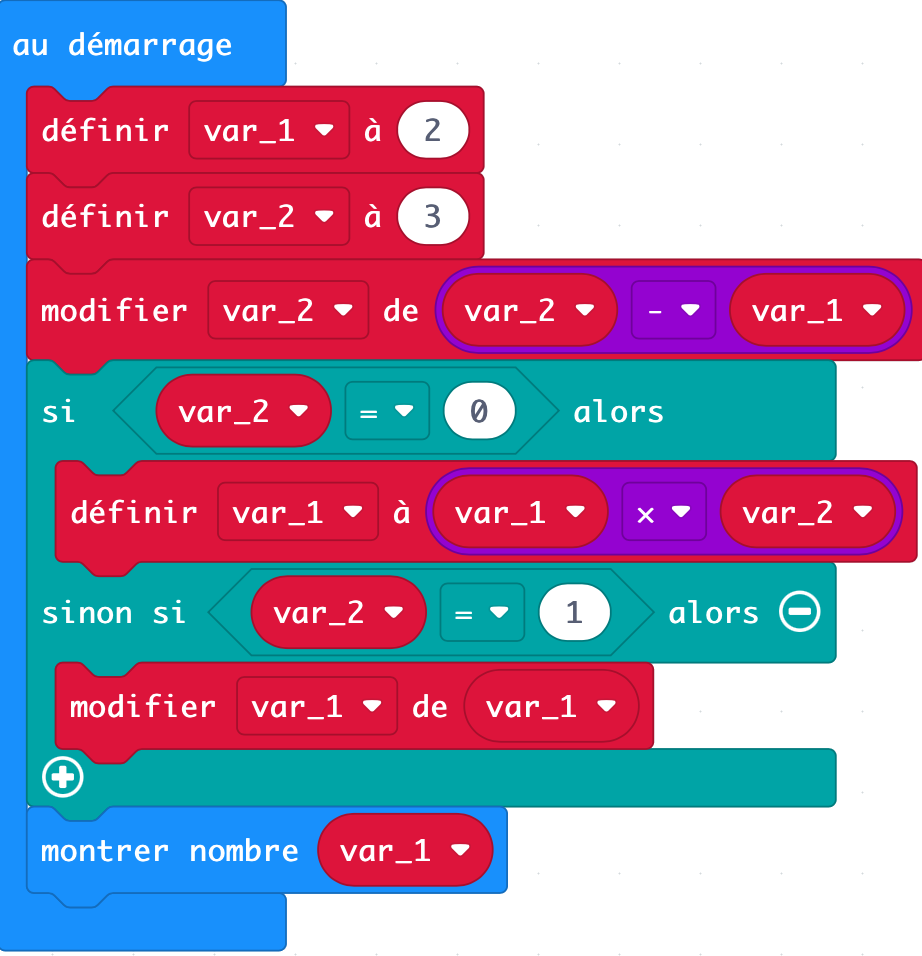
\includegraphics[scale=.5]{ch6_images/var_25}
\end{center}
\end{exercice}

 

\newpage


\begin{exercice}
\begin{center}
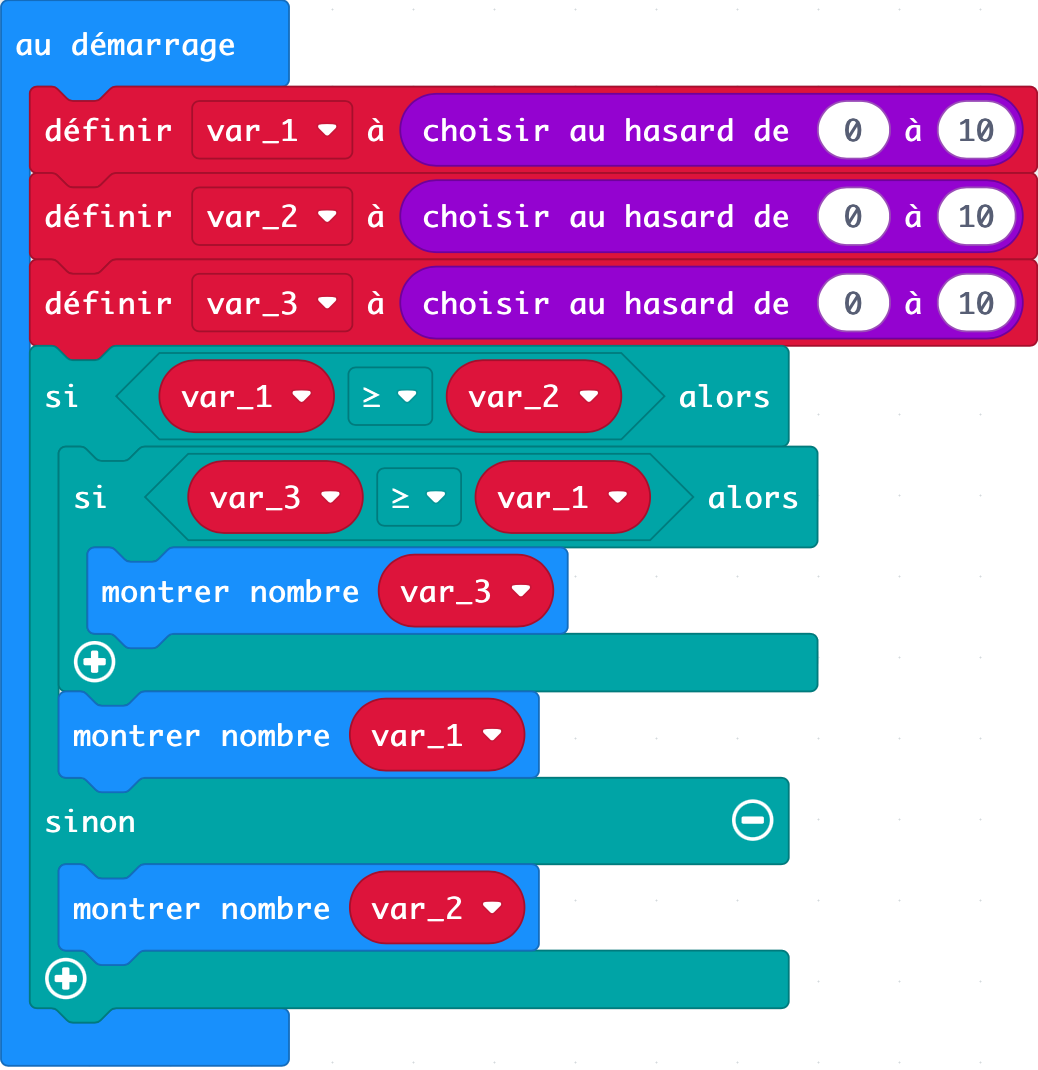
\includegraphics[scale=.5]{ch6_images/var_26}
\end{center}
Que fait ce programme si:
\begin{enumerate}
	\item $var\_1=5$, $var\_2=9$  et $var\_3=2$? 
	\item $var\_1=7$, $var\_2=3$  et $var\_3=3$?
	\item $var\_1=3$, $var\_2=5$  et $var\_3=6$? 
	\item $var\_1=4$, $var\_2=4$  et $var\_3=4$?  
\end{enumerate}
\end{exercice}


\subsection{La boucle {\it répéter} (repeat)}

La condition {\it si} est une structure  nous permettant de coder des conditions mais elle n'est pas suffisante. Pour certain problème, nous avons besoin de répéter une certain nombre de fois une action. Le nombre de répétition peut-être connue à l'avance ou ne pas l'être.

Nous aimerions, par exemple, doubler la valeur de $var\_1$ 5 fois de suite. La première possibilité est la suivante:

\begin{center}
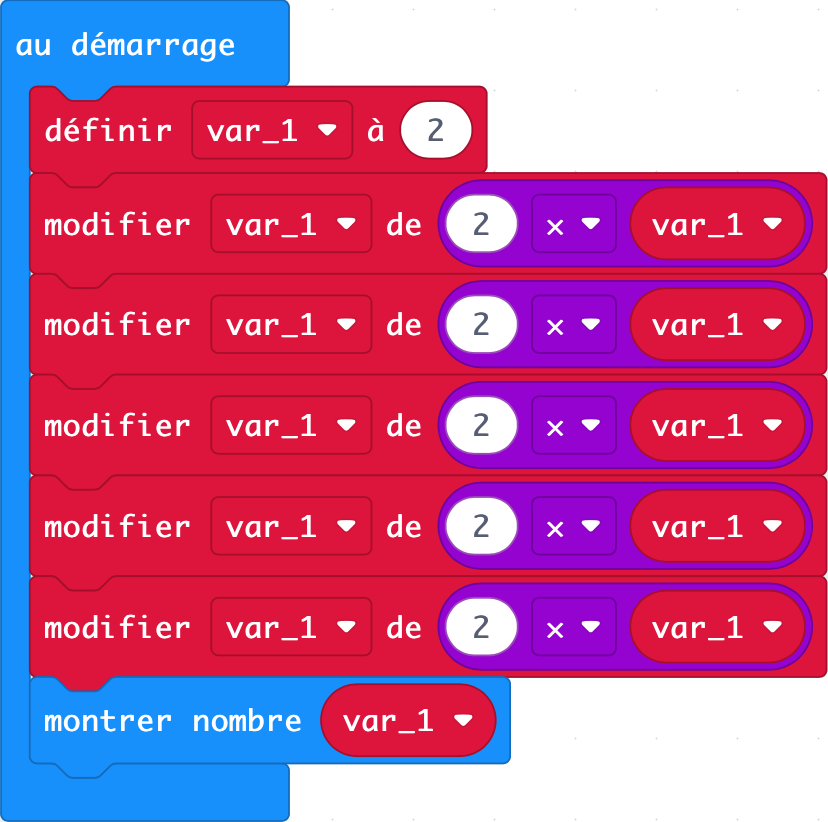
\includegraphics[scale=.5]{ch6_images/var_27}
\end{center}

Lorsque nous répétons plusieurs fois la même action, il est plus facile d'utiliser une boucle {\it répéter} (repeat), qui effectuera une même tâche un certain nombre de fois:

\begin{center}
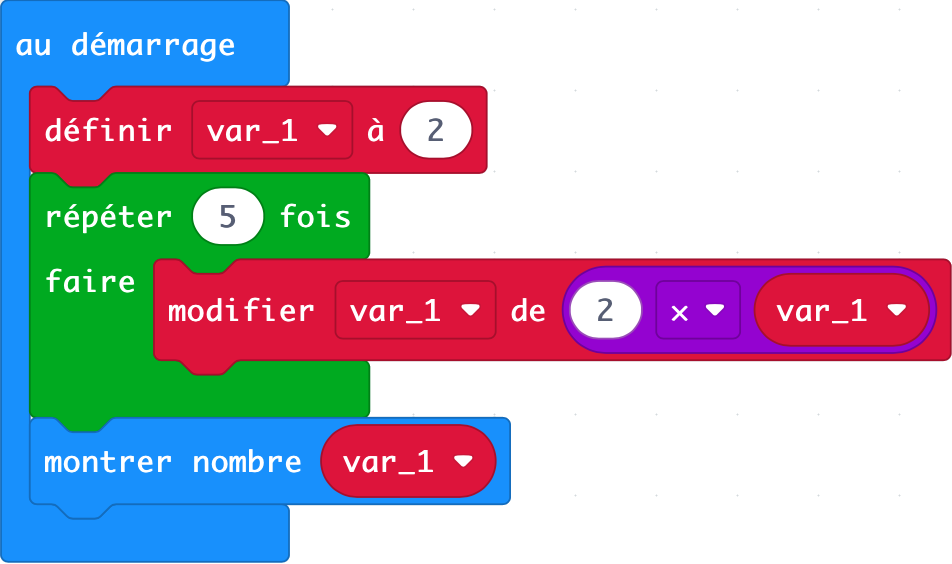
\includegraphics[scale=.5]{ch6_images/var_28}
\end{center}

L'intérêt de {\it répéter} est que nous pouvons aussi utiliser une variable pour le nombre de fois que nous voulons répéter une tâche et donc obtenir une grande flexibilité dans notre programme.

\begin{exercice}
Que fait le programme suivant?
\begin{center}
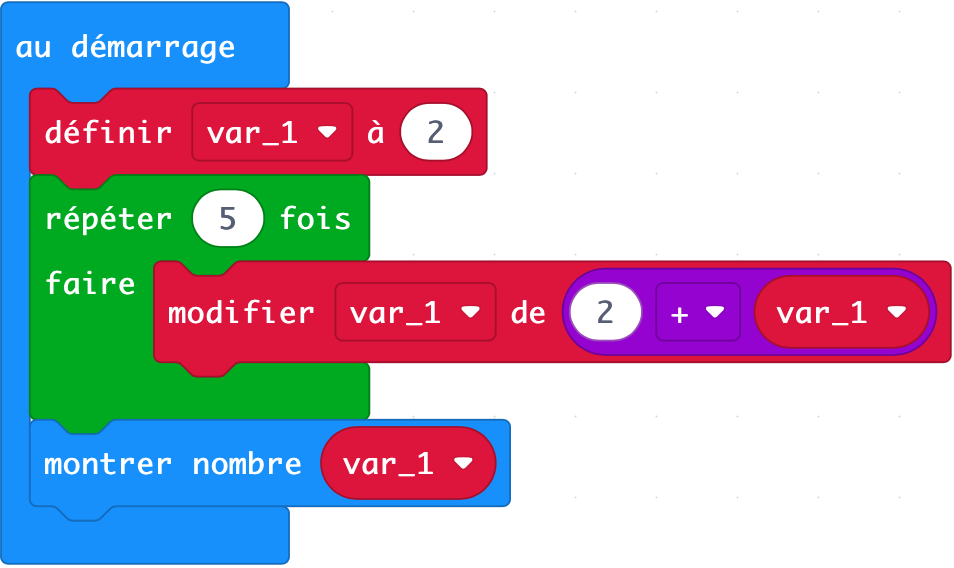
\includegraphics[scale=.5]{ch6_images/var_29}
\end{center}
\end{exercice}


\begin{exercice}
Que fait le programme suivant?
\begin{center}
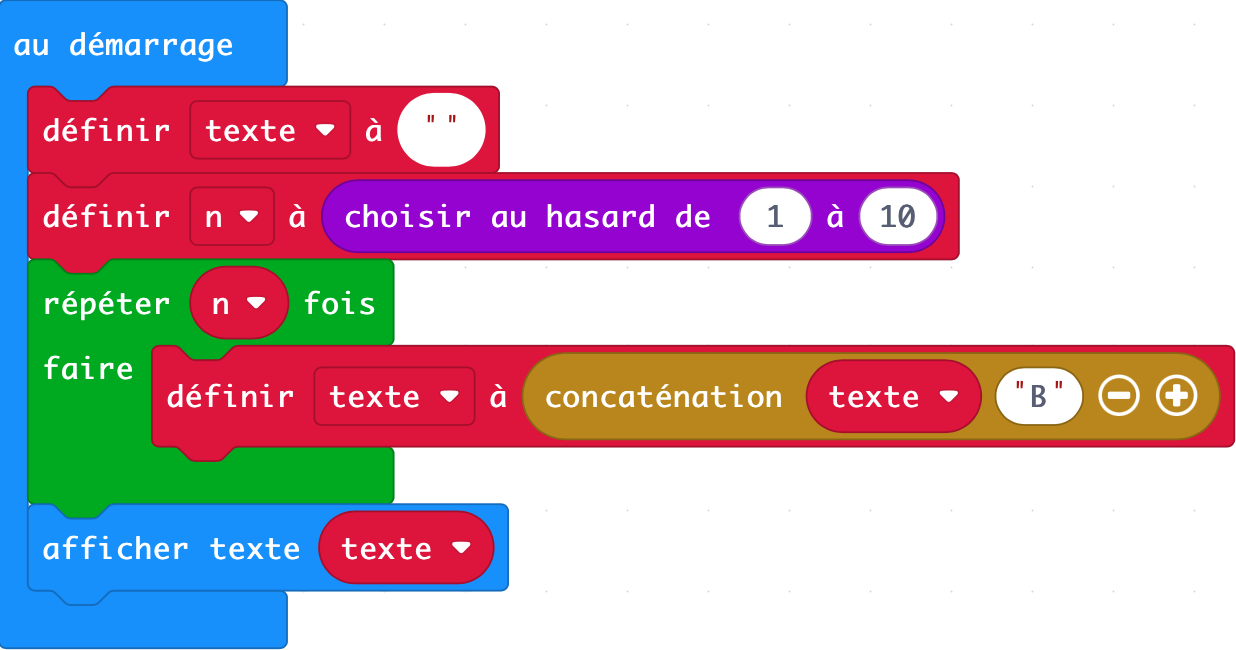
\includegraphics[scale=.5]{ch6_images/var_30}
\end{center}
\end{exercice}


\begin{exercice}
\begin{enumerate}
\item Que fait ce programme si {\it flocon\_x} = 2?
\item Que fait ce programme si {\it flocon\_x} = 4?
\end{enumerate}
\begin{center}
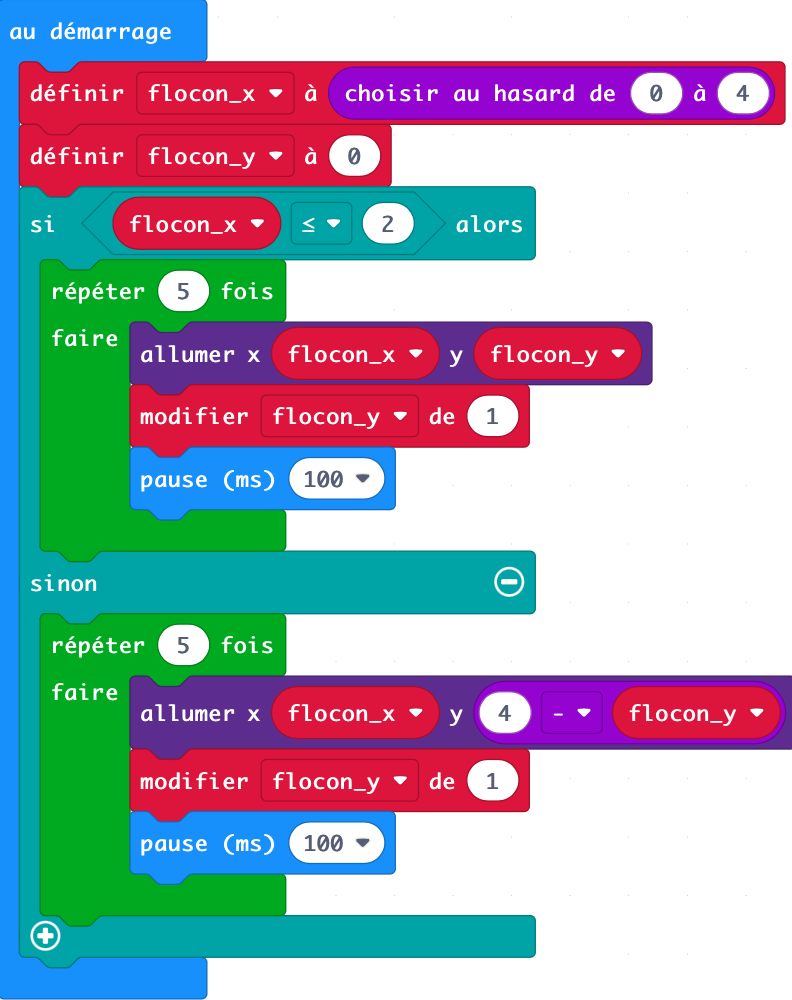
\includegraphics[scale=.5]{ch6_images/var_31}
\end{center}
\end{exercice}

\subsection{La boucle {\it tant que} (while)}

{\it répéter} est une structure de répétition qui ne nous permet pas de faire "efficacement" toutes les répétitions, ou boucle, que nous rencontrons en programmation. Pour palier à cette difficulté, deux autres structures se rencontrent souvent: la boucle {\it tant que } (while) et la boucle {\it pour} (for). Nous allons voir dans ce chapitre la première (alors que la deuxième sera étudiée lorsque nous ferons de la programmation en langage {\it python}.

Le format de la boucle {\it tant que} se présente sous la forme:

\ 

\hskip+5cm {\it tant que} {\bf condition est vraie}

\hskip+6cm faire une certaine séquence d'instructions



\vskip+.5cm

La {\bf condition} consiste souvent à vérifier qu'une variable ne dépasse pas une certaine valeur. Il faudra alors {\bf incrémenter} cette variable avant chaque répétition de la boucle. Lorsque cette valeur est dépassée, on sort de la boucle. 

Il est souvent assez facile de passer d'une boucle {\it tant que} à une boucle {\it répéter}. Par exemple,
les deux programmes suivants, utilisant les structures de répétition {\it répéter} et {\it tant que} sont équivalents:

\begin{multicols}{2}
\begin{center}
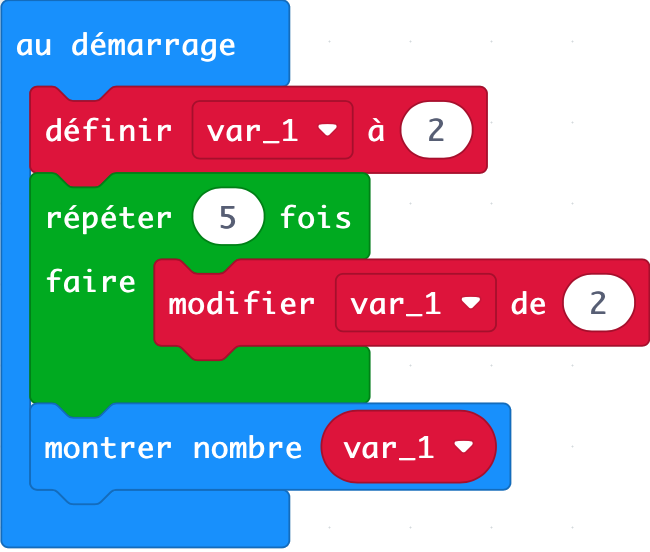
\includegraphics[scale=.5]{ch6_images/var_32}
\end{center}

\begin{center}
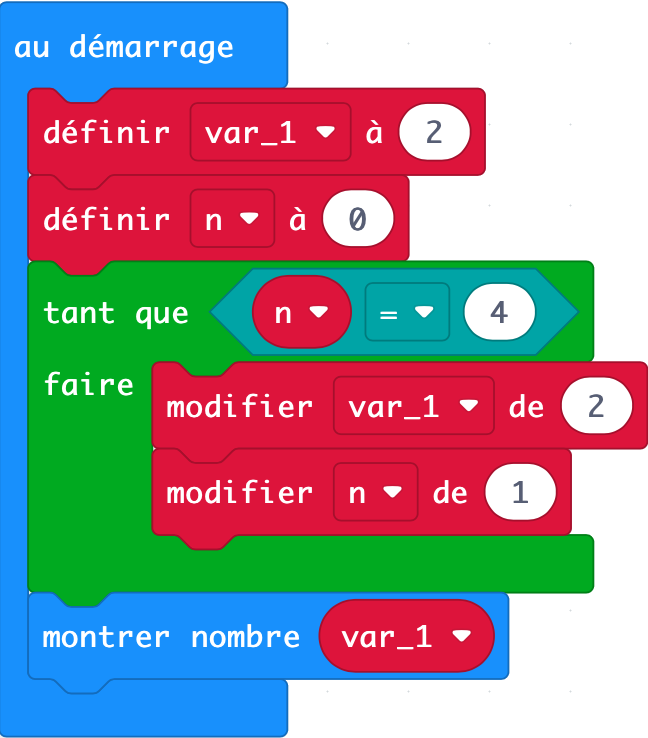
\includegraphics[scale=.5]{ch6_images/var_33}
\end{center}
\end{multicols}

\begin{exercice}
Que fait le programme suivant?
\begin{center}
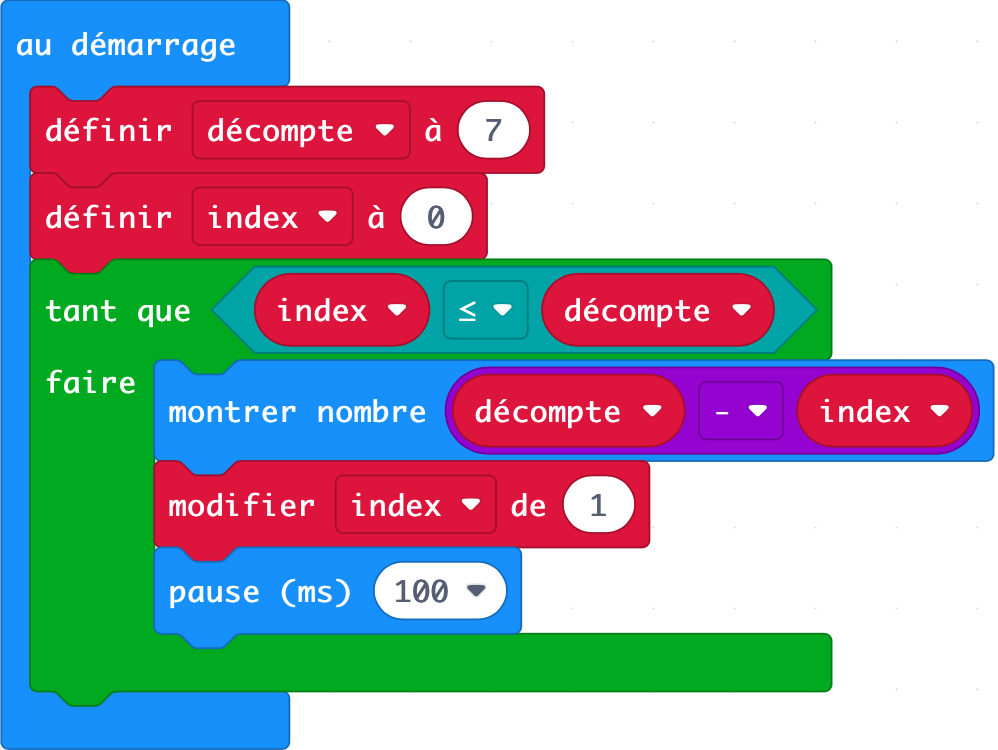
\includegraphics[scale=.5]{ch6_images/var_34}
\end{center}
\end{exercice}

\begin{exercice}
Que fait le programme suivant?
\begin{center}
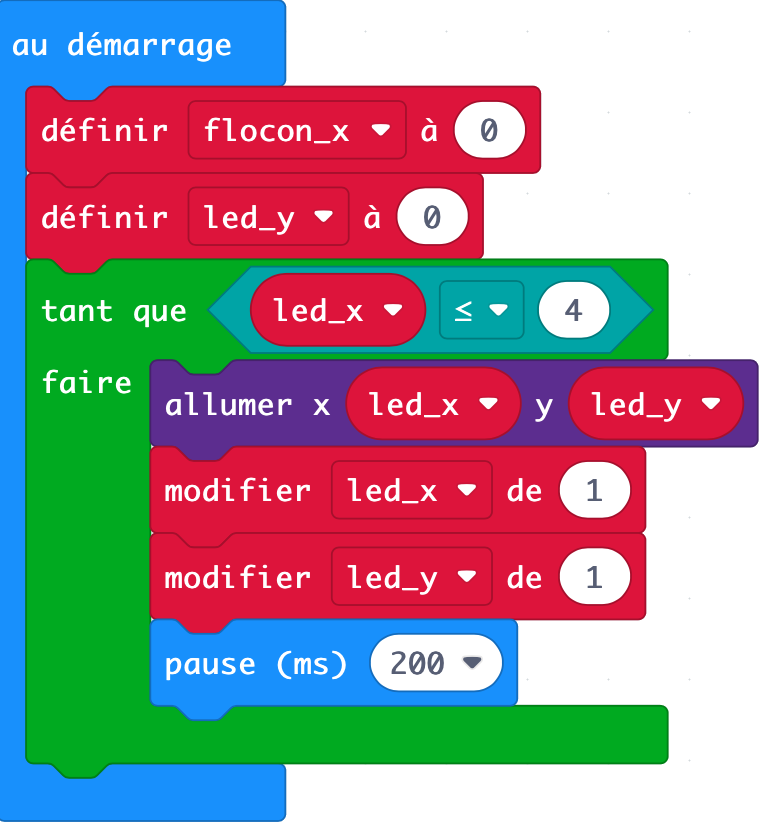
\includegraphics[scale=.5]{ch6_images/var_35}
\end{center}
\end{exercice}

\begin{exercice}
Que fait le programme suivant?
\begin{center}
\includegraphics[scale=.5]{ch6_images/var_36}
\end{center}
\end{exercice}

\end{document}

